%!TEX root = 00-main.tex
\section{Introduction}\label{sec:intro}
\iffalse
I suggest to organize the introduction as follows:
\begin{itemize}
    \item Para 1: Why the interpretabiliy of DNNs is important; Introduce the recent breakthrough NTK; Point out the limitations of NTK (the performance gap between NTK and NNs)
    \item Para 2: Introduce the follow-ups of NTK which tries to handle the limitations of NTK, such as NTH, and their limitations (not applicable)
    \item Para 3: Highlight our argument that another crucial reason is that NTK cannot capture the label information. Show the theoretical analysis in feature space and some specific examples in experiments (I will add the figures later, cat vs dog, bench vs table). 
    \item Para 4: Introduce our generic label-aware kernel and two specific algorithms.
    \item Para 5: Highlight the experimental results and how the results corroborate our proposals.
    \item Para 6: Highlight the implications of our work (or contributions)
\end{itemize}

\fi
%\hangfeng{Add motivated experiments to highlight the importance of label information}
%\sxc{Para 1: Why the interpretabiliy of DNNs is important; Introduce the recent breakthrough NTK; Point out the limitations of NTK (the performance gap between NTK and NNs)}
The last decade has witnessed the huge success of deep neural networks (NNs) in various machine learning tasks \citep{lecun2015deep}. Contrary to its empirical success, however, the theoretical understanding of real-world NNs is still far from complete, hindering its applicability to many domains where interpretability is of great importance, such as autonomous driving and biological research \citep{doshi2017towards}. 

%%\wjs{give some references?} 
%%has been developing positive evidence towards understanding the dynamics of training NNs, via relating to  
%%if we randomly initialize a NN and train it with gradient flow using the least squares loss, then the evolution of the function value $f(\rvx, \rvtheta_t)$ follows the 

More recently, a venerable line of work relates overparametrized NNs to kernel regression from the perspective of their training dynamics, providing positive evidence towards understanding the optimization and generalization of NNs \citep{jacot2018neural,chizat2018note,cao2019generalization,lee2019wide,arora2019exact,chizat2019lazy,du2019graph,li2019enhanced,zou2020gradient}. To briefly introduce this approach, let $\rvx_i, y_i$ be the feature and label, respectively, of the $i$th data point, and consider the problem of minimizing the squared loss $\frac1n\sum_{i=1}^n (y_i - f(\rvx_i, \rvtheta))^2$ using gradient descent, where $f(\rvx, \rvtheta)$ denotes the prediction of NNs and $\bm w$ are the weights. Starting from an random initialization, researchers demonstrate that the evolution of NNs in terms of predictions  can be well captured by the following kernel gradient descent
\begin{equation}
	\label{eq: grad_flow_f}
	\frac{d}{dt}f(\rvx, \rvtheta_t) = - \frac{1}{n} \sum_{i = 1}^n {K (\rvx, \rvx_i)} \bigl(f(\rvx_i, \rvtheta_t) - \rvy_i\bigr)
\end{equation}
in the infinite width limit, where $\rvtheta_t$ is the weights at time $t$. Above, $K(\cdot, \cdot)$, referred to as \emph{neural tangent kernel} (NTK), is time-independent and associated with the architecture of the NNs. As a profound implication, an infinitely wide NNs is ``equivalent'' to kernel regression with a {deterministic kernel} in the training process.

Despite its immense popularity, many questions still remain unanswered concerning the NTK approach, with the most crucial one, perhaps, being the non-negligible performance gap between a kernel regression using the NTK and a real-world NNs. Indeed, according to an experiment done by \cite{arora2019exact}, on the CIFAR-10 dataset \citep{krizhevsky2009learning}, a vanilla 21-layer CNN can achieve $75.57\%$ accuracy, whereas the corresponding convolutional NTK (CNTK) can only attain $64.09\%$ accuracy. This significant performance gap is widely recognized to be attributed to the \textit{finiteness} of widths in real-world NNs. This perspective has been investigated in many papers \citep{hanin2019finite,huang2019dynamics,bai2019beyond,bai2020taylorized}, where various forms of ``finite-width corrections'' have been proposed. However, the computation of these corrections all involve incremental training. This fact is in sharp contrast to kernel methods, whose computation is ``one-shot'' via solving a simple linear system.


%\footnote{In some papers, NTK refers to the time dependent kernel $\KK_t$.}. 
%This notion of equivalence is further generalized in a series of follow-up works \citep{yang2019scaling,arora2019exact,du2019graph,li2019enhanced}. 
% %%A recent paper by \cite{jacot2018neural} has demonstrated the following intriguing fact: 
% They further showed that if the NN is wide enough, then 
% %\begin{equation}
% %	\label{eq: ntk_is_deterministic_when_infinite_width}
% 	$\KK_t \approx \KK_0 \approx \bbE_\init\KK_0,$
% %\end{equation}
% where $\bbE_\init$ is the expectation w.r.t. the random initialization. 
% \emph{Is NTK the best kernel one can possibly design for ``simulating'' the behaviors of NNs?}
% %\end{center}
% To answer this question, let us note a structural property behind the complicated formula of NTK: $\bbE_\init\KK_0$ is \emph{label-agnostic}, 
% %In this paper, we propose a different yet complementary explanation on this performance gap based on \emph{label-awareness}. 

In this paper, we develop a new approach toward closing the gap by recognizing a recently introduced phenomenon termed \textit{local elasticity} in training neural networks~\citep{he2019local}. Roughly speaking, neural networks are observed to be locally elastic in the sense that if the prediction at a feature vector $\bm x$ is not significantly perturbed, after the classifier is updated via stochastic gradient descent at a (labeled) feature vector $\bm x$ that is dissimilar to $\bm x'$ in a certain sense. This phenomenon implies that the interaction between two examples is heavily contingent upon whether their labels are the same or not. Unfortunately, the NTK construction is clearly independent of the labels, thereby being label-agnostic, meaning that it is independent of the labels $\rvy$ in the training data. This ignorance of the label information can cause huge problems in practice, especially when the semantic meanings of the features crucially depends on the \emph{label system}. 


%The NTK theory has successfully explained many previous ``mysteries'' of a NN, such as its capability of interpolating the training data, regardless of the label distribution \citep{zhang2016understanding}. However, many questions still remain unanswered, with the most crucial one, perhaps, being the non-negligible performance gap between a kernel regression using the NTK and a real-world NN. Indeed, according to an experiment done by \cite{arora2019exact}, on the CIFAR-10 dataset \citep{krizhevsky2009learning}, a vanilla 21-layer CNN can achieve $75.57\%$ accuracy, whereas the corresponding convolutional NTK (CNTK) can only attain $64.09\%$ accuracy. 

%\sxc{Para 2: Introduce the follow-ups of NTK which tries to handle the limitations of NTK, such as NTH, and their limitations (not applicable)}

%. 
%\footnote{Recall that for kernel regression, the prediction has an explicit formula which is a linear function of the label vector $\rvy$.}.



\begin{figure}[t]
		\centering
		\scalebox{1.0}{
		\subfigure[NTK: init vs trained]{
			\centering
			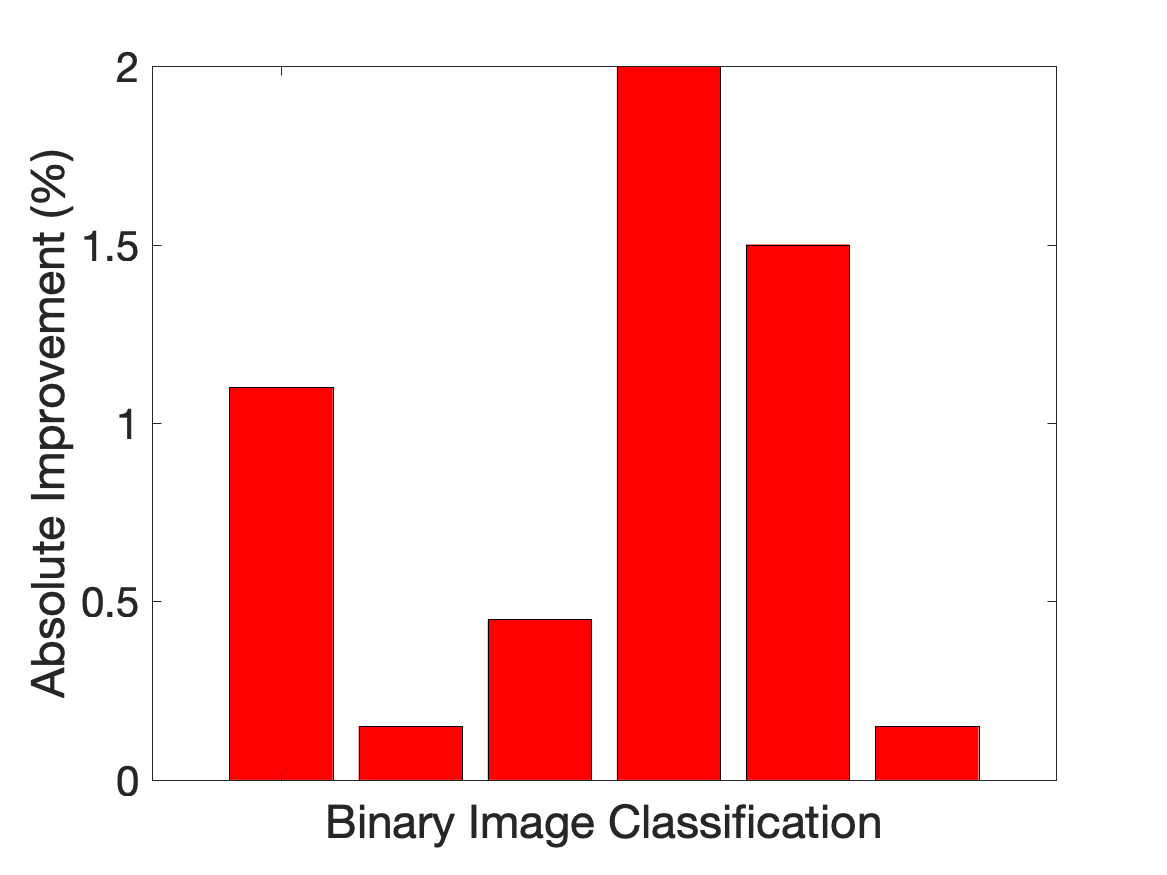
\includegraphics[scale=0.22]{figures/ntk_init_trained.png}
			\label{fig:ntk-init-trained}}
		\subfigure[Local elasticity: cat vs dog]{
			\centering
			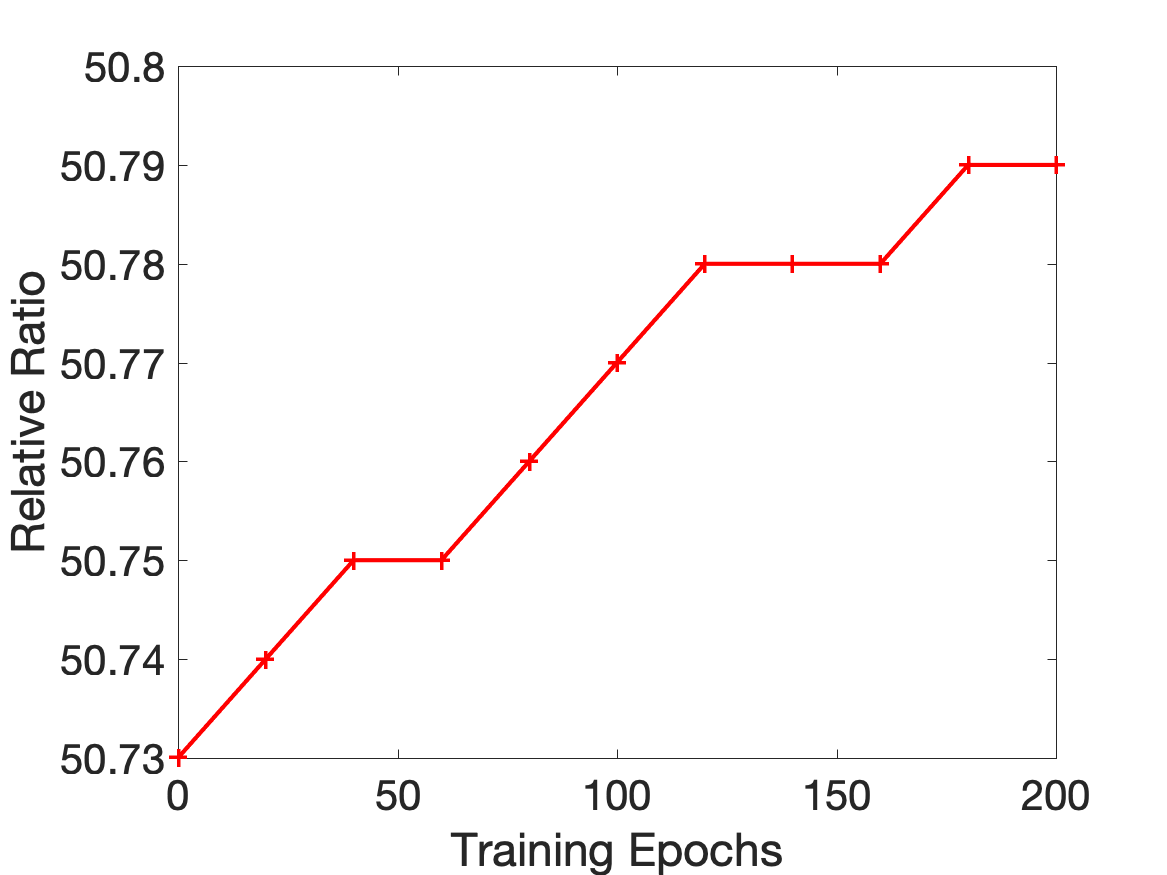
\includegraphics[scale=0.22]{figures/cat_dog_LE.png}
			\label{fig:le-cat-dog}}
        \subfigure[Local elasticity: chair vs bench]{
			\centering
			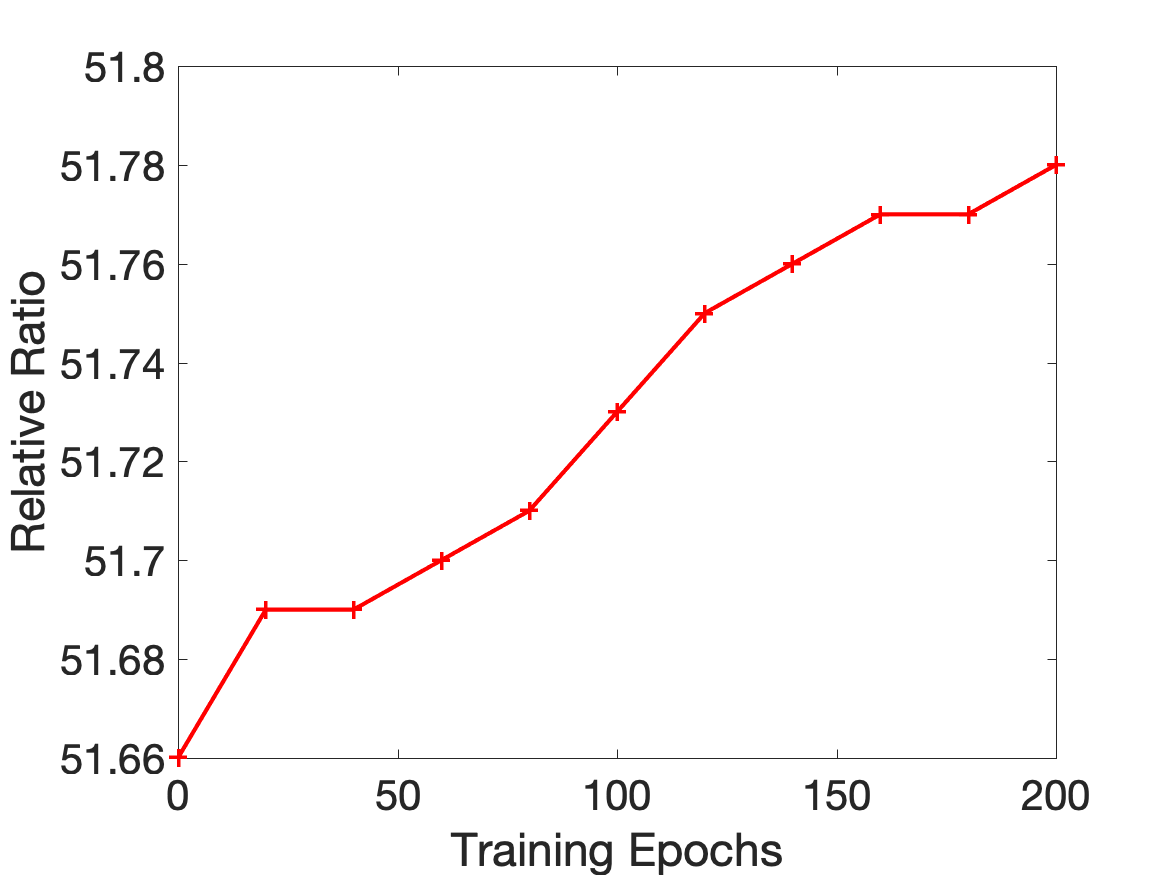
\includegraphics[scale=0.22]{figures/chair_bench_LE.png}
			\label{fig:le-chair-bench}}
		}
        \caption{The impact of labels on a 2-layer NN in the aspect of generalization ability and local elasticity. Fig. (a) displays the absolute improvement in six binary classification tasks by using $\KK_t$ instead of $\KK_0$, indicating that NNs learn better feature representations with the help of labels along the training process (see Sec.~\ref{subsec:local-elasticity} for more details). Fig. (b) and (c) show that in two label systems (cat v.s. dog and bench v.s. chair), the strength of local elasticity (measured by the relative ratio
        %of the kernelized similarity between intra-class examples and inter-class examples, see 
        defined in Eq. \eqref{eq: relative_ratio}) both increases with training, but in different patterns, indicating that the labels play an important role in the local elasticity of NNs (See Appx.~\ref{subsec:different-labeling-systems} for more details).}
		\label{fig:labels-impact}
		\vspace{-17pt}
\end{figure}
%\begin{center}
%\centering


To shed light on the vital importance of the label information, consider a collection of natural images, where in each image, there are two objects: one object is either a cat or dog, and another is either a bench or chair. 
% One can label these images as cat v.s. dog, or one can label them as chair v.s. bench. 
Take an image $\rvx$ that contains dog+chair, and another $\rvx'$ that contains dog+bench. Then for NTK to work well on both label systems, we would need $\bbE_\init K(\rvx, \rvx')  \approx 1$ if the task is dog v.s. cat, and $\bbE_\init K(\rvx, \rvx')  \approx -1$ if the task is bench v.s. chair,
%\begin{align*}
%	\bbE_\init\KK_0(\rvx, \rvx') & \approx 1 \qquad \ \ \ \textnormal{ if the task is dog v.s. cat},\\
%	\bbE_\init\KK_0(\rvx, \rvx') & \approx -1 \qquad \textnormal{ if the task is bench v.s. chair},
%\end{align*}	
a fundamental contradiction that cannot be resolved by the label-agnostic NTK (see also Claim \ref{claim: limitations_of_label_agnostic_kernels}). In contrast, NNs can do equally well in both label systems, a favorable property which can be termed adaptivity to label systems. To understand what is responsible for this desired adaptivity, note that \eqref{eq: grad_flow_f} suggests that NNs can be thought of as a time-varying kernel $\KK_t$. This ``dynamic'' kernel differs from the NTK in that it is \emph{label-aware}, because it depends on the trained parameter $\rvtheta_t$ which further depends on $\rvy$. As shown in Fig. \ref{fig:labels-impact}, such an awareness in labels play an import role in the generalization ability and local elasticity of NNs.

%(a phenomenon specific to NNs observed by \citealt{he2019local}) 
%From the discussion above, it is clear that a kernel regression with $\bbE_\init \KK_0$ alone cannot explain the generalization properties of a NN, since the latter is able to \emph{adapt to} different label systems. 


%The discussion above gives a different yet complementary perspective on the performance gap between NTK and real-world NNs: a kernel regression with NTK alone cannot simulate a NN well because NTK is label-agnostic.
Thus, in the search of ``NN-simulating'' kernels, it suffices to limit our focus on the class of label-aware kernels. 
% This brings a structural question: \emph{what does a generic label-aware kernel look like}? 
% %How to properly incorporate the label information to the NTK so that it becomes adaptive to different label systems, just as the NN does? 
% Mathematically, a generic label aware kernel $K(\rvx, \rvx', S)$ may have arbitrary dependence structure on the training data $S = \{(\rvx_i, \rvy_i): i\in[n]\}$. Fortunately, using \emph{Hoeffding Decomposition} \citep{hoeffding1948class}, we are able to obtain a structural lemma (Lemma \ref{lemma: hoeffding_decomp}), which asserts that any label-aware kernel can be decomposed into the superimposition of a label-agnostic part and a \emph{hierarchy} of label-aware parts with increasing complexity of label dependence. 
%the following formula (see Theorem \ref{thm: hoeffding_decomp}):
%\begin{align}
%	K(\rvx, \rvx', S)& = \gK^{(2)}_\varnothing(\rvx, \rvx') + \sum_{i\in[n]}\gK^{(3)}_i(\rvx, \rvx', \rvy_i) + \sum_{i\neq j}\gK^{(4)}_{ij}(\rvx, \rvx', \rvy_i, \rvy_j) \nonumber \\
%	\label{eq: hoeffding_decomp_layerwise} 
%	& \qquad + \cdots + \gK^{(n+2)}_{[n]}(\rvx, \rvx', \rvy_1, \hdots, \rvy_n) ,
%\end{align}
%where $\{\gK^{(r+2)}_{A}: 0\leq r\leq n , |A| = r\}$ is a collection of functions s.t. $\gK^{(r+2)}_A$ only depends on $\rvy_A = \{\rvy_i:i\in A\}$. That is, any label-aware kernel can be decomposed into the superimposition of a label-agnostic part $\gK^{(2)}_\varnothing$ (the zero-th level), and a \emph{hierarchy} of label-aware parts with increasing complexity on the label dependence --- $\gK^{(3)}_i$'s (the first level) depends on a single label, $\gK^{(4)}_{ij}$'s (the second level) depends on a pair of labels, etc.
\textcolor{black}{In this paper,} we propose two label-aware NTKs (\lantk s). 
% \sout{\textcolor{red}{both of which can be regarded as \emph{truncated versions} of the Hoeffding Decomposition at some finite level.}} 
The first one is based on a notion of \emph{higher-order regression}, which extracts higher-order information from the labels by estimating whether two examples are from the same class or not. The second one is based on approximately solving neural tangent hierarchy (NTH), an infinite hierarchy of ordinary different equations that give a precise description of the training dynamics \eqref{eq: grad_flow_f} \citep{huang2019dynamics}, and we show this kernel approximates $\KK_t$ strictly better than $\bbE_\init \KK_0$ does (Theorem \ref{thm: approx_nth_error}). 

\textcolor{black}{Although the two \lantk s stems from very different intuitions, their analytical formulas are perhaps surprisingly similar: they are both quadratic functions of the label vector $y$. This brings a natural question: \emph{is there any intrinsic relationship between the two?} And more generally, \emph{what does a generic label-aware kernel, $K(\rvx, \rvx', S)$, which may have arbitrary dependence structure on the training data $S = \{(\rvx_i, \rvy_i): i\in[n]\}$, look like?}
Using \emph{Hoeffding Decomposition} \citep{hoeffding1948class}, we are able to obtain a structural lemma (Lemma \ref{lemma: hoeffding_decomp}), which asserts that any label-aware kernel can be decomposed into the superimposition of a label-agnostic part and a \emph{hierarchy} of label-aware parts with increasing complexity of label dependence. And the two \lantk s we developed can, in a certain sense, be regarded as the \emph{truncated versions} of this hierarchy. 
} 
% This brings a structural question: \emph{what does a generic label-aware kernel look like}? 
%How to properly incorporate the label information to the NTK so that it becomes adaptive to different label systems, just as the NN does? 
% Mathematically, a generic label aware kernel $K(\rvx, \rvx', S)$ may have arbitrary dependence structure on the training data $S = \{(\rvx_i, \rvy_i): i\in[n]\}$. 



We conduct comprehensive experiments to confirm that our proposed \lantk s can indeed better simulate the quantitative and qualitative behaviors of NNs compared to their label-agnostic counterpart. On the one hand, they generalize better: the two \lantk s achieve a $1.04\%$ and $1.94\%$ absolute improvement in test accuracy ($7.4\%$ and $4.1\%$ relative error reductions) in binary and multi-class classification tasks on CIFAR-10, respectively. On the other hand, they are more ``locally elastic'': the relative ratio of the kernelized similarity between intra-class examples and inter-class examples increases, a typical trend observed along the training trajectory of NNs. 


\iffalse
%{\noindent \bf Our contributions.} We summarize our contributions below.
\begin{enumerate}[itemsep=0mm]
	\item We propose a different and complementary perspective on why NTK alone cannot explain the generalization properties of NNs based on the notion of \emph{label-awareness}. Specifically, we construct a counterexample showing that if the label-agnostic NTK works well on one label system, then there exists a ``natural relabelling'', on which NTK can work arbitrarily bad. This is in sharp contrast to real-world NNs, which are able to adapt to different label systems.
	\item Using Hoeffding Decomposition, we decompose a generic label-aware kernel into the superimposition of a label-agnostic part and a hierarchy of label-aware parts with increasing complexity of label dependence. 
	\item Inspired by the decomposition, we propose two label-aware versions of NTK. One is based on a notion of \emph{higher-order regression}, and another is based on approximately solving NTH. We also prove that the latter one approximates the time-dependent kernel $\KK_t$ strictly better than $\KK_0$ does. 
	\item We conduct thorough experiments to show that the label-aware versions of NTK can significantly increase the test accuracy compare to its label-agnostic counterpart, and their behaviors more closely resemble those of a neural net. 
\end{enumerate}
\fi
\subsection{Related Work}
{\bf Kernels and NNs.} Starting from \citet{neal1996priors}, a line of work considers infinitely wide NNs whose parameters are chosen randomly and only the last layer is optimized \citep{williams1997computing,le2007continuous,hazan2015steps,lee2017deep,matthews2018gaussian,novak2018bayesian,garriga2018deep,yang2019scaling}. %Under this setup, the function computed by a NN can be described as a Gaussian process. 
When the loss is the least squares loss, this gives rise to a class of interesting kernels different from the NTK. 
%of the following form: $K(\rvx, \rvx') = \bbE_\init [f(\rvx, \rvtheta_0)f(\rvx', \rvtheta_0)]$.
On the other hand, if all layers are trained by gradient descent, infinitely wide NNs give rise to the NTK
%, which takes the following form $K(\rvx, \rvx') = \bbE_\init [\la\partial f(\rvx, \rvtheta_0)/\partial \rvtheta, \partial f(\rvx', \rvtheta_0)/\partial \rvtheta\ra]$ 
\citep{jacot2018neural,chizat2018note,lee2019wide,arora2019exact,chizat2019lazy,du2019graph,li2019enhanced}, and the NTK also appears implicitly in many works when studying the optimization trajectories of NN training \citep{li2018learning,allen2018convergence,du2018gradient,ji2019polylogarithmic,chen2019much}.


{\bf Limitations of the NTK and corrections.} \cite{arora2019harnessing} demonstrates that in many small datasets, models trained by the NTK can outperform its corresponding NN. But for moderately large scale tasks and for practical architectures, the performance gap between the two is empirically observed in many places and further confirmed by a series of theoretical works \citep{chizat2019lazy,ghorbani2019linearized,yehudai2019power,bietti2019inductive,ghorbani2019limitations,wei2019regularization,allen2019can}. This observation motivates various attempts to mitigate the gap, such as incorporating pooling layers and data augmentation into the NTK \citep{li2019enhanced}, deriving higher-order expansions around the initialization \citep{bai2019beyond,bai2020taylorized}, doing finite-width correction \citep{hanin2019finite}, injecting noise to gradient descent \citep{chen2020generalized}, and most related to our work, the NTH~\citep{huang2019dynamics}. 

{\bf Label-aware kernels.} The idea of incorporating label information into the kernel is not entirely new. For example, \cite{cristianini2002kernel} proposes an alignment measure between two kernels, and argues that aligning a label-agnostic kernel to the ``optimal kernel'' $\rvy\rvy^\top$ can lead to favorable generalization guarantees. This idea is extensively exploited in literature on kernel learning (see, e.g., \citealt{lanckriet2004learning,cortes2012l2,gonen2011multiple}). 
%We refer the readers to the awesome review paper \citet{gonen2011multiple} and references therein.
In another related direction, \cite{tishby2000information} proposes the information bottleneck principle, which roughly says that an optimal feature map should simultaneously minimize its mutual information (MI) with the feature distribution and maximize its MI with the label distribution, thus incorporating the label information (see also \citealt{tishby2015deep} in the context of deep learning). 
%\cite{tishby2015deep} uses this principle to study the representations learned in intermediate layers of NNs. 
We refer the readers to Appx. \ref{append:connections} for a detailed discussion of the connections and differences of our proposals to these two lines of research.
